\documentclass[a4paper, 11pt, final, garamond]{book}
\usepackage{cours-preambule}
\usepackage{pdfpages}

\raggedbottom

\makeatletter
\renewcommand{\@chapapp}{Travaux pratiques -- TP}
\makeatother

\let\SavedIndent\indent
\protected\def\indent{%
  \begingroup
    \parindent=\the\parindent
    \SavedIndent
  \endgroup
}
\setlength{\parindent}{0pt}

\begin{document}
\setcounter{chapter}{17}

\chapter{\'Etude de la chute d'une bille en fluide visqueux}

\section{Objectifs}

\begin{itemize}
    \item Savoir enregistrer expérimentalement à l'aide d'une \textit{webcam} le
        mouvement de chute d'un solide dans un autre fluide en vue de
        l'exploitation du document obtenu. Savoir exploiter un résultat
        expérimental.
    \item Reconnaître si le mouvement du centre d'inertie est rectiligne
        uniforme ou non.
    \item Reconnaitre le régime transitoire et le régime permanent.  Déterminer
        la vitesse limite.
    \item Évaluer le temps caractéristique $\tau$ par deux méthodes.
    \item Trouver un ordre de grandeur de la viscosité $\eta$ de l'huile de
        silicone. 
\end{itemize}

\section{S'approprier}

\subsection{Matériel}

\begin{itemize}
    \item Éprouvette contenant l'huile de silicone et des billes
    \item \textit{Webcam}
    \item Ordinateur et logiciel \texttt{Latispro}
    \item Chronomètre
\end{itemize}
   
\subsection{Données}

\begin{itemize}
    \item Bille orange~: $R = \SI{1,0}{cm}$ et $m = \SI{10,4}{g}$.
    \item Masse volumique de l'huile de silicone~: $\rho_0 =
        \SI{970}{kg.m^{-3}}$.
    \item $g = \SI{9,8}{m.s^{-2}}$.
\end{itemize}
 
\subsection{Principe}

\begin{wrapfigure}{r}{0.25\textwidth} 
    \vspace{-210pt}
    \begin{center}
        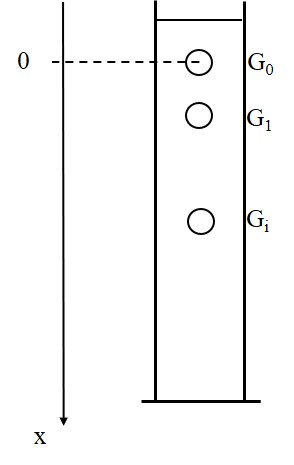
\includegraphics[width=0.2\textwidth]{chute_bille}
    \end{center}
    \vspace{-30pt}
\end{wrapfigure} 

Une éprouvette contenant un liquide visqueux sert de support à l'étude de la
chute d'une bille d'acier. Le schéma ci-dessus donne une idée du montage, et
n'est qu'indicatif. En particulier, il ne respecte pas d'échelle. La bille, qui
constitue le système matériel étudié, est lâchée sans vitesse initiale à
l'instant $t = 0$. 

\bigbreak

Le système d'acquisition vidéo est assuré par une \textit{webcam} couplée à un
ordinateur et réglée de manière à enregistrer 20 images par seconde. La position
instantanée $x$ du centre de gravité G de la bille est repérée par l'axe
vertical $(\Or x)$ orienté vers le bas, de vecteur unitaire $\ux$.
 
\section{Analyser}

On étudie le mouvement de translation d'une bille de rayon $R$ et  de masse
volumique $\rho$ dans de l'huile de silicone de viscosité $\eta$. On admettra
que les actions de frottement exercées par le liquide sur la bille en mouvement
à la vitesse $\vect{v}$ sont modélisables par une force de frottement
$\vect{f}$ telle que 

\[
    \vect{f} = -6\pi \,\eta \, R \, \vect{v}
\]

\bigbreak

On dépose la bille en O sans vitesse initiale dans l'huile de silicone contenue
dans une grande éprouvette. On exprimera  toutes les expressions littérales en
fonction de $\tau_0$, $\eta$, $R$, $m$ et $g$.

\bigbreak

\begin{enumerate}[label=\clenumi]
    \item Donner les caractéristiques de la poussée d'Archimède $\vect{\Pi}$
        exercée sur la bille plongeant dans l'huile de silicone, sachant que
        c'est une force verticale orientée vers le haut, de module égal au
        \textbf{poids du fluide qui serait occupé par le volume de l'objet}.
    \item Faire le bilan des forces exercées sur la bille plongeant dans l'huile
        de silicone en précisant le référentiel de travail.
    \item Établir l'équation différentielle que vérifie la valeur de la vitesse
        $\vect{v}$ du centre d'inertie de la bille, sous la forme~: 
 
        \[
            \dv{v}{t} + \frac{6\pi \eta R}{m}v = g\pa{1-\frac{4\pi \rho_0 \,
            R^3}{3m}}
        \]
    \item Montrer que la vitesse de la bille tend vers une vitesse limite
        $v\ind{limTheo}$  telle que~:

        \[
            v\ind{limTheo} = \frac{g}{6\pi \eta R} \pa{m-\frac{4\pi \rho_0 \, R^3}{3}}
        \]
    \item Donner l'expression de la constante de temps $\tau\ind{theo}$ du
        mouvement en fonction de $m$, $\eta$ et $R$.
    \item En déduire la forme de la solution de l'équation différentielle en $v(t)$. 
\end{enumerate}

\section{Réaliser}
\subsection{Enregistrement vidéo}

\subsubsection{Préréglages de la \textit{webcam} et de la prise de vue}

\begin{enumerate}
    \item Ouvrir le logiciel \texttt{Amcap3} dans Bureau $\ra$ Programmes
        Physique Chimie $\ra$ \texttt{Amcap3}.

    \item dans le menu Options~: 
        \begin{itemize}
            \item \texttt{Preview}, pour visualiser ce qu'on voit dans la
                caméra. Régler la distance caméra-éprouvette pour voir
                uniquement la moitié supérieure de l'éprouvette. Le trait noir
                sur l'éprouvette aide à régler l'horizontal de la caméra. Régler
                l'objectif de la caméra pour que l'image soit nette (faire le
                point sur l'éprouvette).

            \item \texttt{Video capture pin}~: taille de sortie choisir,
                \texttt{640*360}. Fréquence image~: 20. Format~: MJPG.
                $\ra$ Appliquer $\ra$ OK.
            \item \texttt{Video capture filter}~: luminosité, netteté et
                contraste en positions intermédiaires. $\ra$ Appliquer
                $\ra$ OK.
        \end{itemize}
    \item Puis dans le menu \texttt{Capture}.
        \begin{itemize}
            \item \texttt{Set Frame Rate}~: nombre d'images par seconde~: 20.
                $\ra$ Cocher~: \texttt{use} $\ra$ OK.
            \item \texttt{Set time limit}~: \SI{5}{s} $\ra$ Cocher~:
                \texttt{use} $\ra$ OK.
            \item \texttt{Start capture}~: dossier élève~: choisir où vous
                mettez vos dossiers.
        \end{itemize}
\end{enumerate}
 
\subsubsection{Enregistrement de la vidéo}

Aller sur~: \texttt{Capture}~; \texttt{Start Capture}~: Cliquer sur \texttt{OK},
puis lâcher la bille juste après.
 
\subsection{Traitement vidéo de la chute de la bille}

\begin{enumerate}
    \item Ouvrir le logiciel \texttt{Latispro} dans programmes $\ra$
        discipline $\ra$ physique-chimie $\ra$ Eurosmart.
    \item Cliquer sur la 5\ieme\ icône~: lecture de séquence AVI (ressemblant à
        Google chrome).
    \item Fichiers $\ra$ ouvrir le fichier \texttt{avi}.
    \item Revenir à zéro pour exploiter (4\ieme\ icône en bas).
    \item Grâce à >, choisir le début de la vidéo à exploiter (première image
        quand la bille commence à descendre).
    \item Puis cliquer sur sélection de l'origine et pointer la bille, grâce à
        la loupe à droite.
    \item Sélection de l'étalon~: sélection de haut en bas sur la partie visible
        de l'éprouvette.
    \item Indiquer la distance associée (ne pas mettre l'unité qui est le
        \si{m}). $\ra$ correspond à la hauteur de l'éprouvette graduée.
    \item Sens des axes~: \fbox{$\downarrow \ra$}. Sélection manuelle des
        points.
    \item Viser la cible et pointer grâce au zoom à droite~: pointer alors ainsi
        une quarantaine de positions de la bille.
    \item Terminer la sélection manuelle, quand il y a assez de points.
    \item Fermer la fenêtre. Pour exploiter, cliquer sur le signal sinusoïdal
        vert. Icône~: \fbox{$\sim$}.
\end{enumerate}

\section{Valider et conclure}

\subsection{Exploitation du traitement vidéo}

\subsubsection{Tracé de la vitesse verticale en fonction du temps}

\begin{itemize}
    \item Traitements~: $\ra$ Calculs spécifiques. $\ra$ Dérivée. $\ra$ Faire
        glisser $y$ pour obtenir $v = \dv{y}{t}$
    \item Pour visualiser $v = f(t)$, faire glisser la fonction $v$ sur le
        graphe. On affichera uniquement les points sans les relier. 
\end{itemize}

\subsubsection{Modélisation de la vitesse}
\begin{itemize}
    \item Cliquer modéliser.
    \item Choisir le modèle sous forme $A(1-\exr^{-t/\tau})$ (forme théorique
        attendue pour la loi de vitesse d'après la partie s'approprier). On
        forcera $V_0 = 0$ sur le modèle. Le calculer.
    \item Le glisser sur la courbe en superposition.
    \item Pour afficher la modélisation~: Copier dans le presse papier $\ra$
        Fermer $\ra$ Créer un commentaire $\ra$ Coller après avoir choisi une
        fenêtre.
\end{itemize}

\subsubsection{Détermination de la vitesse limite}

\begin{enumerate}[label=\sqenumi, start=7]
    \item À partir de la modélisation, déterminer la valeur expérimentale de la
        vitesse limite.
\end{enumerate}

\subsubsection{Détermination de la constante de temps $\tau$ par deux méthodes}

\textit{i - Utilisation du temps de montée} \bigbreak

\begin{enumerate}[label=\sqenumi, resume]
    \item Quelle est la valeur de la vitesse (en pourcentage de la vitesse
        limite $v_{\lim}$) lorsque $t=\tau$~? En déduire une méthode de
        détermination de $\tau$ (qui est celle du cours). 
\end{enumerate}
\begin{itemize}
    \item Utiliser le pointeur, par clic droit sur la fenêtre graphique.
\end{itemize}
\begin{enumerate}[label=\sqenumi, resume]
    \item Relever $\tau\ind{exp1}$. Recliquer droit pour terminer.
\end{enumerate}

\bigbreak

\textit{ii - Utilisation de la modélisation de la vitesse} \bigbreak

\begin{enumerate}[label=\sqenumi, resume]
    \item Déduire de la modélisation de la vitesse l'ordre de grandeur de la
        constante de temps $\tau\ind{exp2}$.
    \item Calculer l'écart normalisé entre les deux valeurs expérimentales de
        $\tau$. L'écart normalisé n'est pas l'écart relatif.
\end{enumerate}
 
\subsubsection{Détermination de la viscosité $\eta$ de l'huile de silicone}

\begin{enumerate}[label=\sqenumi, resume]
    \item Grâce à l'étude théorique de la partie S'approprier et à la valeur
        moyenne de $\tau\ind{exp}$, déterminer la valeur expérimentale de la
        viscosité $\eta\ind{exp}$ en précisant son unité.
    \item La comparer à la valeur théorique de la viscosité $\eta\ind{theo} =
        \SI{1,5}{SI}$.
\end{enumerate}
 
\subsection{Détermination plus rapide de la vitesse limite sans enregistrement vidéo}
\subsubsection{Protocole expérimental}

\begin{enumerate}[label=\sqenumi, resume]
    \item Justifier que le régime transitoire ait une durée négligeable devant
        la durée totale de chute de la bille.
    \item Proposer alors puis réaliser un protocole expérimental (sans
        enregistrement) qui permettrait de déterminer la vitesse limite en
        répétant les mesures 5 à 6 fois.
    \item Partagez vos résultats de mesure avec le reste de la classe.
    \item En déduire une nouvelle valeur de $v_{\lim}$, en tenant compte de vos
        différents mesurages et de ceux des autres groupes de la classe. Vous
        présenterez le résultat avec l'incertitude élargie pour un intervalle de
        confiance à $95 \%$.
\end{enumerate}

\subsubsection{Incertitude de répétabilité (type A) et écriture du résultat}

Lorsqu'on répète plusieurs fois le mesurage de la même grandeur, dans les mêmes
conditions expérimentales, on peut trouver des résultats légèrement différents.
Il en est de même pour des opérateur-ces différent-ess réalisant simultanément
le mesurage de la même grandeur avec du matériel similaire. Dans de tels cas, on
utilise des notions de statistiques pour analyser les résultats. \bigbreak

L'incertitude de mesure correspondant à des mesures répétées d'une même grandeur
est appelée incertitude de répétabilité (type A). Chaque groupe effectuera 5
mesures indépendantes de $v_{\lim}$. Les valeurs seront toutes affichées au
tableau. Ainsi, chaque groupe pourra utiliser toutes les valeurs de $v_{\lim}$
trouvées (environ 50 valeurs normalement, mais vous pourrez vous limiter à une
vingtaine de valeurs) pour déterminer le mesurage de $v_{\lim}$ selon la
formule que l'on rappelle ici~: 

\begin{timpo}{Rappel}
    \[
        M(v_{\lim}) = \obar{m}(v_{\lim}) \pm U(v_{\lim})
        \qqet
        U(v_{\lim}) = \frac{2}{\sqrt{n}} \sqrt{\frac{1}{n-1}
            \, \sum_{i=1}^{n} (m_i(v_{\lim})-\obar{m}(v_{\lim}))^2}
    \]
    $U(v_{\lim})$ représente ici l'incertitude élargie pour un intervalle de
    confiance de $95 \%$. 
\end{timpo}

\begin{rexem}{Remarque}
    La grandeur $\sqrt{\frac{1}{n-1} \, \sum_{i=1}^{n}
    (m_i(v_{\lim})-\obar{m}(v_{\lim}))^2}$ représente l'écart-type non biaisé
    sur vos calculatrices. 
\end{rexem}

\end{document}
